% I2AI 26/27-F ara sınav ödevi: A1–A4'ü raporlayan IEEE konferans bildirisi.
% Şablon: dersin değiştirilmiş IEEE A4 şablonu (conference-template-a4_w-notes_I2AI-2627F.docx).
% Derleme: tectonic Pair24_EightBits_Midterm.tex  (ya da Overleaf, pdfLaTeX; şekiller: python figures.py)
\documentclass[conference,a4paper]{IEEEtran}
\usepackage[T1]{fontenc}
\usepackage{newtxtext,newtxmath}
\usepackage{cite}
\usepackage{amsmath}
\usepackage{graphicx}
\usepackage{array}
\usepackage{url}
% Şablonun Word sürümü "Keywords—" yazar; IEEEtran'ın varsayılanı "Index Terms".
\renewcommand{\IEEEkeywordsname}{Keywords}
% Erişilebilirlik: PDF üstverisi, belge dili ve tıklanabilir bağlantılar; görünüm değişmez (hidelinks).
\usepackage[hidelinks]{hyperref}
\hypersetup{pdftitle={I2AI 26/27-F AI-agent Project: Abalone Case Study},
  pdfauthor={Salih Eren, Eren Terakye},
  pdfsubject={Abalone agent: search, adversarial search and learning (I2AI 26/27-F midterm paper)},
  pdfkeywords={Abalone, game-playing agent, alpha-beta search, temporal-difference learning},
  pdflang={en-US}}

\begin{document}

\title{I2AI 26/27-F AI-agent Project:\\ Abalone Case Study}

% Şablondaki biçim: tek satırda yazarlar, altında bölüm ve üniversite, sonra e-postalar.
% E-postalar: yazarların kurumsal öğrenci adresleri.
\author{\IEEEauthorblockN{Salih Eren, Eren Terakye}
\IEEEauthorblockA{\textit{Department of Computer Engineering, Eskisehir Osmangazi University}, Eskişehir, Türkiye\\
152120231091@ogrenci.ogu.edu.tr, 152120231068@ogrenci.ogu.edu.tr}}

\maketitle

\begin{abstract}
In the board game Abalone, each player tries to push six of the opponent's fourteen marbles off a hexagonal board of 61 cells. We report an Abalone agent developed over the four assignments of an introductory artificial intelligence course. We define the task environment, formulate the game as a search problem on bitboards, compare uninformed, informed, local, and online search on single-agent sub-problems, and plan against every opponent reply with AND-OR search. The final agent is a utility-based learning agent that selects moves by alpha-beta search with iterative deepening, a transposition table, move ordering, killer moves, and quiescence search, while temporal-difference learning in self-play tunes its six evaluation weights; logistic regression and a small value network serve as alternative learners. A later rewrite searches exactly as before but about five times faster; with half a second per move it beats the presented version in 82 of 100 games and our previous agent in all 50. Minimax without pruning and Monte Carlo tree search with the same evaluation win only 2 of 100 games against it. Ablations show that the learned weights and quiescence search contribute most, and that better outcome prediction by a supervised model did not yield stronger play.
\end{abstract}

\begin{IEEEkeywords}
Abalone, adversarial search, alpha-beta pruning, game-playing agent, heuristic search, reinforcement learning
\end{IEEEkeywords}

\section{Introduction}
Artificial intelligence can be studied as the design of rational agents, which select the action expected to maximize their performance measure given their percepts~\cite{russell2021}. Board games suit this view, because their rules define the environment exactly while their size rules out exhaustive analysis, so an agent must decide with limited lookahead.

Abalone is played on a hexagonal board of 61 cells with 14 black and 14 white marbles; Black moves first. A move shifts one to three own marbles in a line by one cell, along the line (in-line) or sideways (broadside). An in-line group may push a smaller opposing group (sumito: two against one, three against one or two) if the cell beyond it is empty or off the board, and the first player to push six opposing marbles off wins.

The problem addressed here is to choose, in a given position and within a fixed time per move, the legal move that maximizes the chance of winning against an opponent who plays to the contrary. Three properties make it hard. The branching factor is about 60 in typical play~\cite{lemmens2005}, against about 35 in chess~\cite{russell2021}. Human games last 87 plies on average~\cite{lemmens2005}, which gives roughly $60^{87}\approx5\times10^{154}$ move sequences over at most $2\times10^{25}$ board configurations by our count, against the $10^{24}$--$10^{25}$ estimated in~\cite{chorus2009}. Finally, the rules do not force progress: a cautious player can keep its marbles away from the edge indefinitely.

We built the agent over the four assignments of the course. Beyond summarizing them, this paper compares the methods on common benchmarks, measures the final agent against its predecessors, its own ablations, and the alternatives in Chapter~6 of~\cite{russell2021} in controlled matches, and contrasts reinforcement and supervised learning of the same evaluation. Section~II covers the environment and the methods (Chapters 2--4, 6, 19, 22, and 23 of~\cite{russell2021}), Section~III the agent and its results, and Section~IV concludes.

\section{Material \& Methods}

\subsection{Task Environment}
Table~\ref{tab:peas} gives the performance measure, environment, actuators, and sensors (PEAS) of the agent and the properties of its task environment~\cite{russell2021}; the marble margin, pushed off minus lost, ranks wins. Being fully observable, deterministic apart from the opponent's choice, and known, the environment needs neither belief states nor exploration; being competitive and sequential, it requires planning against the opponent. A simple reflex agent cannot look ahead, a model-based one gains nothing from tracking hidden state, and a goal-based one cannot compare the many middle-game moves that reach no goal, so we designed a utility-based agent, which ranks the predicted states $\textsc{Result}(s,a)$ of its actions by a utility $U$~\cite{russell2021}, and later made it a learning agent.

\begin{table}[!b]
\caption{Task Environment of the Abalone Agent}
\label{tab:peas}
\centering
\footnotesize
\begin{tabular}{@{}>{\raggedright\arraybackslash}p{0.78in}>{\raggedright\arraybackslash}p{2.53in}@{}}
\hline
\textbf{PEAS} & \textbf{Description} \\
\hline
Performance & Win (six marbles off), ranked by marble margin; legal moves only, each within the time budget \\
Environment & 61-cell hexagonal board, 14 marbles per side, the opponent, the turn order \\
Actuators & Move 1--3 marbles in-line or broadside; sumito push \\
Sensors & Board, side to move, opponent's last move, marbles off \\
\hline
\textbf{Property} & \textbf{Value} \\
\hline
Observable & Fully observable \\
Agents & Multi-agent, competitive \\
Deterministic & Deterministic; only the opponent's choice is open \\
Episodic & Sequential \\
Static & Static; semi-dynamic with a clock \\
Discrete & Discrete \\
Known & Known \\
\hline
\end{tabular}
\end{table}

\subsection{Problem Formulation and Abstraction}
A state is a pair of 61-bit integers $(P,O)$ holding the cells of the side to move and of its opponent; bit $i$ stands for cell $i$, and a precomputed table gives the neighbor of every cell in each of the six directions. This bitboard abstraction keeps only occupancy and packs a state into 16 bytes. The initial state is the standard layout. $\textsc{Actions}(s)$ returns every legal in-line, broadside, and sumito move; $\textsc{Result}(s,a)$ moves and pushes the marbles, drops a marble pushed past the edge, and swaps $P$ and $O$. The terminal test is that one side has eight marbles left or, under the match rules of Section~III-B, the game is drawn; the utility is $+1$, $0$, or $-1$, and every move costs 1. Two independently written move generators agreed on 2,000 random positions and both give the perft counts 44, 1,936, and 98,912 from the opening.

The search algorithms of Chapter~3 of~\cite{russell2021} assume a single agent, so Assignment~2 defined a sub-problem: with the opponent's marbles frozen as pushable obstacles, push one of them off in the fewest moves. Sixty puzzles with optimal length $d^{*}\in\{2,3,4\}$ were generated by random walks from the opening. Two admissible heuristics were derived by relaxation. The rim-distance heuristic ignores our marbles: since a move pushes at most two opposing marbles one cell each, $h_R(s)=\max\bigl(r,\lceil(e_1+\dots+e_r)/2\rceil\bigr)$, where $r$ push-offs are still needed and $e_1\le e_2\le\dots$ are the distances of the opposing marbles to leaving the board. The formation heuristic adds that two of our marbles must line up behind the target, $h_F(s)=\max\bigl(h_R(s),\min_{p,c}\,1+\max(t_c,\delta_{pc})\bigr)$, where $\delta_{pc}$ is the distance of opposing marble $p$ to edge cell $c$ and $t_c$ the moves our nearest marbles need to form a pushing pair behind $c$. The heuristic $h_F$ dominates $h_R$, never overestimated $d^{*}$, and violated consistency on none of 103,125 transitions.

\subsection{Search Strategies}
On the sub-problem we benchmarked breadth-first search (BFS), uniform-cost search (UCS), greedy best-first search, A*~\cite{hart1968}, and iterative deepening A* (IDA*)~\cite{korf1985}, limited to $10^{6}$ generated nodes (IDA*: $2\times10^{6}$). UCS tests for the goal on expansion rather than generation, so with unit costs it generates up to $b$ times more nodes than BFS. Depth-first, depth-limited, and iterative deepening search (IDS) were analyzed on the opening's game tree, where IDS to depth 4 re-expanded only 2.0\% more nodes than one depth-limited pass at linear memory; bidirectional search does not apply, as the goal is a predicate, not a state.

\subsection{Search in Complex Environments}
Assignment~3 applied local search to 200 new puzzles of the same kind, climbing on $-h_F$: steepest-ascent, stochastic, and first-choice hill climbing (HC), stochastic HC with up to 20 restarts, HC with up to 100 sideways moves, and simulated annealing~\cite{kirkpatrick1983} with $T(t)=2\cdot0.995^{t}$; learning real-time A* (LRTA*)~\cite{korf1990} represented online search. Belief states were analyzed but are not needed in a fully observable game; an agent seeing only the cells within distance 2 of its marbles would face 31,824 boards in the test position.

The key result of Assignment~3 concerned the opponent, whose reply a plan cannot choose. AND--OR search~\cite{russell2021} treats our moves as OR nodes and the replies as AND nodes and returns a contingent plan; we used it to decide whether the side to move can force $n$ push-offs within $m$ own moves without losing a marble. On the test position of Assignment~3, greedy play on $U$ chose a quiet move after which 7 of the 43 replies prevent any capture, whereas AND--OR search proved that exactly one of the 73 first moves forces two push-offs within two moves, answering 37 of the 39 replies with one move and the other two with their own. The Assignment~3 agent therefore played greedily on $U$ but took a forcing move whenever one existed.

\subsection{Adversarial Search}
The final agent searches the game tree with minimax in negamax form, pruned by alpha--beta~\cite{knuth1975}. Iterative deepening deepens the search until the time runs out, plays the best move of the deepest completed iteration, and reorders the root moves by the previous values. Since alpha--beta prunes most when good moves come first, it tries the transposition-table move first, then moves that push a marble off, two killer moves per ply~\cite{akl1977}, other pushes, and the rest by the history heuristic~\cite{schaeffer1989}. The transposition table stores the depth, value, bound type, and best move of every searched position $(P,O)$. Quiescence search evaluates only quiet positions~\cite{russell2021}: at the depth limit, moves that push a marble off are searched for up to six more plies, with the static value as a lower bound, so that no position is judged in the middle of an exchange. A root move back to a position seen earlier in the game is valued as a draw.

Leaves are evaluated by the linear utility
\begin{equation}
U(s) = \sum_{i=1}^{6} w_i\, f_i(s), \label{eq:u}
\end{equation}
where each feature is the difference between the side to move and the opponent, which makes $U$ antisymmetric, as negamax requires. The features are the marble count; centrality, the sum over marbles of 4 minus the ring index (0 at the center, 4 on the edge); cohesion, the number of adjacent own pairs; edge marbles; exposed marbles, edge marbles touching an opposing marble; and wedges, marbles flanked by opposing marbles on one line. The first four form the utility of Assignment~1 and match features of earlier Abalone agents~\cite{ozcan2004,lemmens2005}; the last two address weaknesses noted in~\cite{lemmens2005}. The features are divided by fixed scales (1, 10, 10, 5, 5, and 3) so that one learning rate suits all weights, and the hand-set weights $\mathbf{w}=(10,20,10,-15,0,0)$ reproduce the Assignment~1 utility.

\subsection{Learning the Evaluation Function}
Assignment~4 replaced the hand-set weights in~(\ref{eq:u}) by learned ones and compared three learners. TDLeaf($\lambda$)~\cite{baxter2000}, used by the final agent, extends temporal-difference learning~\cite{sutton1988,tesauro1995} to search: the value of a position is its alpha--beta value, and the gradient is taken at the principal-variation leaf whose static evaluation produced that value. With $v_t$ the search value at ply $t$ for Black, the predicted result is $r_t=\tanh(v_t/K)$ with $K=30$, the final $r_N$ is the reward $R$, and each game yields the update
\begin{equation}
\Delta\mathbf{w} = \alpha \sum_{t=1}^{N-1} \nabla_{\mathbf{w}} r_t \sum_{j=t}^{N-1} \lambda^{\,j-t}\,(r_{j+1}-r_j), \label{eq:tdleaf}
\end{equation}
where $\nabla_{\mathbf{w}} r_t=(1-r_t^{2})\,\sigma_t\,\mathbf{f}(l_t)/K$, $\sigma_t=\pm1$ for Black or White to move, and $\mathbf{f}(l_t)$ holds the features of the leaf $l_t$. The reward is $R=\pm1$ for a win by six push-offs and $\tanh(\Delta m/2)$ otherwise, $\Delta m$ being Black's marble lead after a repetition or at the 200-ply cap. We ran 150 iterations of 8 parallel games (1,200 games, 383~s on 8 cores) at depth 2 with $\alpha=10$ and $\lambda=0.7$, averaging the updates~(\ref{eq:tdleaf}) within each iteration and starting from the hand-set weights and four random opening plies.

Logistic regression~\cite{russell2021,buro1995}, the supervised counterpart, labels each quiet position of a finished game, one without an available push-off, with the result $z$ for the side to move (1, 0.5, or 0) and fits $E[z\mid s]=\sigma\bigl(\sum_i \beta_i f_i(s)\bigr)$ without intercept, as the features are antisymmetric. Since $\tanh(v/K)=2\sigma(2v/K)-1$, the evaluation weights are $w_i=\beta_i K/2$. The data were 1,200 self-play games of the hand-set agent at depth 2, split by game into 960 training games (54,153 positions) and 240 test games (13,006 positions). The value network~\cite{russell2021} replaces the features by the raw board: 122 binary inputs, 16 rectified linear hidden units, and a sigmoid output for the expected result of the side to move, 1,985 parameters in all. It was trained on the same positions, holding out 10\% of the training games for early stopping, with each position shown under a random one of the 12 board symmetries.

\section{Agent Type, Performance Analysis, and Discussion}

\subsection{Agent Design and Implementation}
The final agent is a utility-based learning agent~\cite{russell2021}: its percept is the board after the opponent's move, its state the bitboard pair, its decision an alpha--beta search on $U$ with the TDLeaf weights, and its action the chosen move. It is written in pure Python, with a browser interface whose developer mode shows the candidate moves, their values, and the alpha--beta tree; the code, all game records, and a supplementary document with every result are available online~\cite{repo}.

After the presentation, profiling showed 88\% of the search time in the evaluation and the move generator, so we rewrote both without changing the search: the features are computed for all marbles at once from six shifted bitboards, quiescence generates only the moves that push a marble off, and static values are cached. On 386 middle-game positions, the new engine returns the same moves, values, and node counts as the presented one at depths 3 and 4, but 5.5 and 4.5 times faster; with 0.5~s per move it completes 4.1 plies on average instead of 3.3. Thirty-four automated tests check this equivalence, the perft counts, and that alpha--beta returns the minimax value; timed results below use the new engine.

\subsection{Experimental Protocol}
A match has 50 games unless stated otherwise: random two-ply openings, alternating between the standard and Belgian Daisy layouts, each played twice with colors swapped. A game ends when six marbles are off, when a position occurs for the third time (a draw), or after 200 plies, when the side with more marbles wins. Results are given as wins--draws--losses (W--D--L) and as the score $(W+D/2)/N$ for $W$ wins and $D$ draws in $N$ games, with a 95\% normal-approximation confidence interval (CI) whose half-width is at most 0.14 for 50 games. Unless stated otherwise, both players get 0.5~s per move. The new matches ran 24 games in parallel on a 12-core laptop; the Assignment~4 matches ran on a faster computer, so engines are compared only within one run.

\subsection{Search Strategies on the Sub-Problems}
Table~\ref{tab:search} summarizes the sub-problem experiments; the supplementary material gives them in full. BFS solved 58 of the 60 puzzles within the limit; UCS, testing late, solved 28 and generated 47 times more nodes than BFS at $d^{*}=2$. A* with $h_R$ behaved like BFS, since $h_R=1$ whenever an opposing marble is within two cells of leaving the board. A* with $h_F$ solved all puzzles optimally with 3.4, 30.7, and 60.0 times fewer nodes than BFS at $d^{*}=2$, 3, and 4, its effective branching factor falling to 29.0, 13.4, and 10.5 against 54.1, 42.6, and 29.6. Greedy search needed 92 times the optimal number of moves, and IDA* matched A* with at most five states in memory.

\begin{table}[!b]
\caption{Single-Agent Search on Push-Off Puzzles}
\label{tab:search}
\centering
\footnotesize
\setlength{\tabcolsep}{3.5pt}
\begin{tabular}{@{}lrrrr@{}}
\hline
\textbf{Method} & \textbf{Solved} & \textbf{Optimal} & \textbf{Nodes}$^{\mathrm{a}}$ & \textbf{Moves}$^{\mathrm{b}}$ \\
\hline
\multicolumn{5}{@{}l}{\textit{Assignment 2: 60 puzzles, at most $10^{6}$ generated nodes}} \\
BFS & 58 & 58 & 79,189 & 2.71 \\
UCS & 28 & 28 & 912,543$^{\mathrm{c}}$ & 2.32 \\
A*, $h_R$ & 58 & 58 & 79,207 & 2.71 \\
A*, $h_F$ & 60 & 60 & 2,582 & 2.75 \\
Greedy, $h_F$ & 60 & 8 & 21,972 & 251.8 \\
IDA*, $h_F$ & 60 & 60 & 3,348 & 2.75 \\
\hline
\multicolumn{5}{@{}l}{\textit{Assignment 3: 200 puzzles}} \\
A*, $h_F$ & 200 & 200 & 5,165 & 2.96 \\
Steepest-ascent HC & 16 & 16 & 101 & -- \\
HC, sideways moves & 194 & 17 & 2,473 & 25.25 \\
Simulated annealing & 200 & 0 & 234 & 218.12 \\
LRTA* & 110 & 17 & 34,448 & 217.93 \\
\hline
\end{tabular}\\[1pt]
\parbox{\columnwidth}{\scriptsize $^{\mathrm{a}}$Assignment~2: mean generated nodes on the 37 puzzles with $d^{*}=3$; Assignment~3: mean evaluations (A*: generated nodes). $^{\mathrm{b}}$Mean solution length; Assignment~3: on the 106 puzzles solved by all four methods with a value. $^{\mathrm{c}}$Includes runs stopped at the limit.}
\end{table}

In local search, steepest-ascent hill climbing stopped on 184 of the 200 puzzles, always on a plateau and never at a strict local minimum; 167 of the plateaus were shoulders. Sideways moves raised the success rate to 97\%, at 25.25 moves per solution against 2.96 for A*, and annealing and LRTA* needed over 200 moves; since every extra move hands the opponent a turn, local search plans poorly in this game. Hill climbing on the Assignment~1 utility raised $U$ from 26 to 100 in 17 moves from the opening without touching an opposing marble, and on the 200 puzzles 76.5\% of the climbs on $U$ never pushed a marble off: the hand-set $U$ rewards a fortress that never attacks.

\subsection{Final Agent Against Earlier Agents}
Under equal time, the final agent beat the Assignment~3 agent 50--0--0 (Table~\ref{tab:matches}; 48--2--0 with the presented engine), 48 games by six push-offs. Alpha--beta search alone accounts for most of this margin, as the hand-set alpha--beta agent also beat it 49--1--0. Against the presented engine, with the same weights and clock, the new engine scored 0.85 (82--6--12) in 100 games: the deeper search alone makes the agent clearly stronger.

\begin{table}[!t]
\caption{Match Results for Player A Against Player B}
\label{tab:matches}
\centering
\footnotesize
\setlength{\tabcolsep}{2.9pt}
\begin{tabular}{@{}llccc@{}}
\hline
\textbf{Player A} & \textbf{Player B} & \textbf{Budget} & \textbf{W--D--L} & \textbf{Score (95\% CI)} \\
\hline
Final agent & A4 engine$^{\mathrm{b}}$ & 0.5 s & 82--6--12 & 0.85 (0.78--0.92) \\
Final agent & A3 agent & 0.5 s & 50--0--0 & 1.00 (0.93--1.00)$^{\mathrm{c}}$ \\
Hand-set $U$ & A3 agent & 0.5 s & 49--1--0 & 0.99 (0.97--1.00) \\
Minimax & Final agent & 0.5 s & 2--3--45 & 0.07 (0.01--0.13) \\
MCTS & Final agent & 0.5 s & 0--0--50 & 0.00 (0.00--0.07)$^{\mathrm{c}}$ \\
\hline
TDLeaf & Hand-set & depth 2 & 47--2--1 & 0.96 (0.91--1.00) \\
TDLeaf & Hand-set & depth 3 & 44--5--1 & 0.93 (0.87--0.99) \\
\hline
Logistic & Hand-set & depth 2 & 38--12--0 & 0.88 (0.82--0.94) \\
Logistic & TDLeaf & depth 2 & 9--10--31 & 0.28 (0.17--0.39) \\
Logistic, refit$^{\mathrm{a}}$ & TDLeaf & depth 2 & 24--12--14 & 0.60 (0.48--0.72) \\
Value network & TDLeaf & depth 2 & 0--3--47 & 0.03 (0.00--0.06) \\
Network, refit$^{\mathrm{a}}$ & TDLeaf & depth 2 & 2--3--45 & 0.07 (0.01--0.13) \\
\hline
\end{tabular}\\[1pt]
\parbox{\columnwidth}{\scriptsize $^{\mathrm{a}}$Trained on the 1,200 self-play games of TDLeaf, not of the hand-set agent. $^{\mathrm{b}}$The agent exactly as presented in Assignment~4, same weights; 100 games, all other rows 50. $^{\mathrm{c}}$Wilson interval, as the normal approximation collapses when all games end alike.}
\end{table}

\subsection{Ablation and Search Cost}
Fig.~\ref{fig:ablation} shows equal-time matches between the full agent and copies with one component removed. Both engines rank the components alike: the learned weights matter most (0.85 with the new engine), followed by quiescence search (0.69), move ordering (0.63), and the transposition table (0.59), the last two in 200 games, whereas removing the killer moves made no difference even in 200 games (0.50). Table~\ref{tab:cost} gives the cost at fixed depth; the node counts are the same for both engines. Pruning saves the most: minimax needs 24 times more nodes than alpha--beta at depth 2 and 90 times more at depth 3, a gap that widens with every ply~\cite{knuth1975}. Without move ordering, which keeps only the table move and the root order of the previous iteration and thereby also disables killer moves, depth 4 needs 3.2 times more nodes, which under a fixed budget costs about a ply of lookahead. The transposition table saves 15\% of the nodes at depth 4 and 3\% at depth 3, and killer moves add little once the history heuristic orders the quiet moves. Quiescence search doubles the node count but adds only 20--27\% to the time, as its nodes generate only push-offs, and it ranks second because a static value taken in the middle of a push exchange misleads the search.

\begin{figure}[!b]
\centering
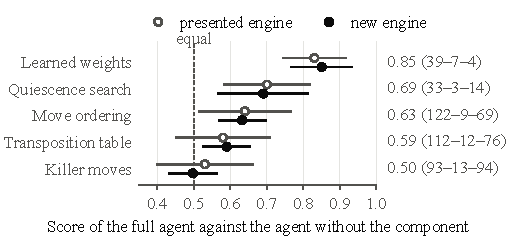
\includegraphics[width=\columnwidth]{fig/ablation.pdf}
\caption{Equal-time ablation (0.5 s per move): score of the full agent against a copy without one component, with 95\% confidence intervals. Hollow: presented engine, 50 games. Filled: new engine, 200 games for the three search enhancements and 50 otherwise, with wins--draws--losses at the right. A score above 0.5 means that the component helps.}
\label{fig:ablation}
\end{figure}

\begin{table}[!b]
\caption{Mean Search Cost over 386 Middle-Game Positions}
\label{tab:cost}
\centering
\footnotesize
\begin{tabular}{@{}lrrrr@{}}
\hline
 & \multicolumn{2}{c}{\textbf{Depth 3}} & \multicolumn{2}{c}{\textbf{Depth 4}} \\
\textbf{Configuration} & \textbf{Nodes} & \textbf{Time (ms)} & \textbf{Nodes} & \textbf{Time (ms)} \\
\hline
Full agent & 7,773 & 22.4 & 27,480 & 166.9 \\
No move ordering & 12,811 & 38.2 & 87,516 & 425.6 \\
No transposition table & 8,032 & 22.9 & 32,305 & 215.3 \\
No killer moves & 7,861 & 23.0 & 28,955 & 171.4 \\
No quiescence search & 3,881 & 18.7 & 14,543 & 131.9 \\
No pruning (minimax) & 699,884 & 3,178.5 & -- & -- \\
\hline
\end{tabular}
\end{table}

\subsection{Learning Results}
In Fig.~\ref{fig:learning}(a), the first TDLeaf checkpoint, after 120 self-play games, already scored 0.93 against the hand-set weights, and the final weights scored 0.96 at depth 2 and 0.93 at depth 3. Fig.~\ref{fig:learning}(b) and Table~\ref{tab:weights} show what was learned: the marble weight more than doubled, the edge penalty shrank from $-15$ to $-6.5$, and the two new features took the expected signs. Self-play thus valued captures more and passive safety less than we had, turning the hand-set fortress into an attacker. A run of 3,200 games with a decaying step size did not play better (20--7--23 at depth 2 against the 1,200-game weights), and its edge and exposed weights kept drifting under three seeds: the two features are correlated (0.71), so play constrains their difference only weakly. Weights trained with a result-only reward played even with the marble-reward weights (25--1--24), although self-play without intermediate rewards was reported to stall in Abalone~\cite{campos2003}.

\begin{figure}[!b]
\centering
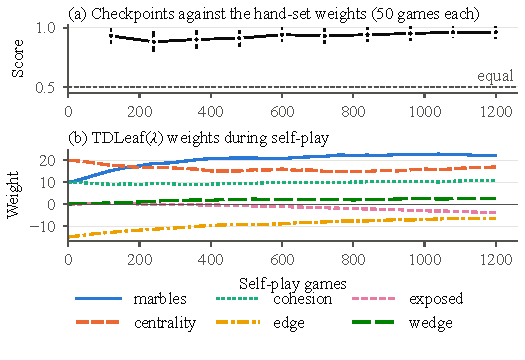
\includegraphics[width=\columnwidth]{fig/learning.pdf}
\caption{TDLeaf($\lambda$) self-play at depth 2. (a) Score of each saved weight vector against the hand-set weights, 50 games each, with 95\% confidence intervals. (b) The six weights on the scaled features during the 1,200 games; Table~\ref{tab:weights} lists the final values.}
\label{fig:learning}
\end{figure}

\begin{table}[!t]
\caption{Evaluation Weights and Held-Out Prediction Quality}
\label{tab:weights}
\centering
\footnotesize
\setlength{\tabcolsep}{4pt}
\begin{tabular}{@{}lrrrr@{}}
\hline
\textbf{Feature} & \textbf{Hand-set} & \textbf{TDLeaf} & \textbf{Logistic} & \textbf{Logistic, refit} \\
\hline
Marbles & 10.0 & 22.1 & 16.3 & 9.2 \\
Centrality & 20.0 & 17.0 & 13.6 & 11.8 \\
Cohesion & 10.0 & 10.8 & $-0.7$ & 3.2 \\
Edge & $-15.0$ & $-6.5$ & 2.8 & 1.3 \\
Exposed & 0.0 & $-3.9$ & $-5.6$ & $-3.4$ \\
Wedge & 0.0 & 2.4 & $-0.7$ & $-0.9$ \\
\hline
Test log loss$^{\mathrm{a}}$ & 0.574 & 0.523 & 0.511 & -- \\
Test accuracy$^{\mathrm{a}}$ & 79.1\% & 83.1\% & 85.5\% & -- \\
\hline
\end{tabular}\\[1pt]
\parbox{\columnwidth}{\scriptsize $^{\mathrm{a}}$13,006 positions of 240 held-out games; accuracy on decisive positions; fixed weight sets scaled by one factor fitted on the training games. Value network: 0.523 and 83.3\%; coin flip: 0.693.}
\end{table}

Predicting outcomes and playing well proved to be different goals. Logistic regression predicted the held-out games best (Table~\ref{tab:weights}) and the network matched TDLeaf, yet in play they lost to TDLeaf 9--10--31 and 0--3--47. Trained on the games of the passive hand-set agent, half of which reached the ply cap, logistic regression learned a negative cohesion weight and a positive edge weight: a fair summary of those games, but a poor guide for choosing moves. Refitted on TDLeaf's own games, it played even with TDLeaf (0.60), so what reinforcement learning mainly added was generating its own relevant training games. The network still lost after refitting (0.07), probably because 1,985 parameters need far more data than 42,113 correlated positions.

\subsection{Comparison with Alternative Approaches}
AND--OR and alpha--beta search answer different questions: in 529 positions from 60 held-out games of the hand-set agent where AND--OR search could force a push-off within two moves but not at once, the depth-3 final agent chose a forcing move in 286 (54\%), preferring by its own evaluation a better continuation in the rest, so the final agent needs no AND--OR override. The alternatives of Chapter~6 were measured with the final agent's own evaluation and clock (Table~\ref{tab:matches}). Minimax without pruning searches every reply and completes only two plies in 0.5~s, against four for alpha--beta; it scored 0.07. Monte Carlo tree search~\cite{russell2021}, with UCB1 selection and leaves valued by the agent's quiescence search instead of random playouts, which in Abalone can last 4,000 plies~\cite{chorus2009}, lost all 50 games, on average within 70 plies: its 12,120 iterations per move are spread over some 60 moves and their replies, whereas alpha--beta proves most of them irrelevant. This agrees with the 60 wins of alpha--beta over Monte Carlo search in~\cite{chorus2009}. AlphaZero-style learning~\cite{silver2018} would need orders of magnitude more computation. The study is limited by self-made opponents, 50-game matches that resolve only differences of about 0.12, frequent ply-cap endings, and a pure-Python engine that reaches about four plies, so we claim no expert strength.

\section{Conclusion}
We built an Abalone agent because the game pairs a precisely known, fully observable environment with a search space far too large for exhaustive analysis, a clear setting in which to test the methods of the course against each other. Informed search with a relaxed heuristic was the only reliable planner on the sub-problems, AND--OR search gave guarantees against every reply, and alpha--beta search with quiescence search and self-play weights beat our previous agent, minimax, and Monte Carlo tree search by wide margins; a faster engine with the same search was clearly stronger still.

The agent's main benefit is transparency: its developer mode makes every decision inspectable, which suits teaching search, and every claim about it rests on logged experiments. Its risks are that its strength was measured only against our own agents and that learned weights can be poorly determined, so a learned evaluation must be validated by play. Future work includes a compiled engine, external opponents, and larger self-play networks.

\section*{Acknowledgment}
This study was carried out within the scope of the 152117107 Introduction to Artificial Intelligence course at Eskisehir Osmangazi University, under the supervision of Asst.~Prof.~Savaş Okyay. Claude Opus 5.5 (Anthropic) helped with the code, text, and experiments, and Gemini (Google) checked the references (supplementary Section~S8); the authors reviewed all content and take full responsibility for it.

\bibliographystyle{IEEEtran}
\bibliography{refs}

\end{document}
